\phantomsection
\addcontentsline{toc}{chapter}{\numberline{}Appendix}
\chapter*{Appendix}

\phantomsection


\appendix

\section*{CODA API}
\label{appendix:CodaAPI}
\begin{figure}
	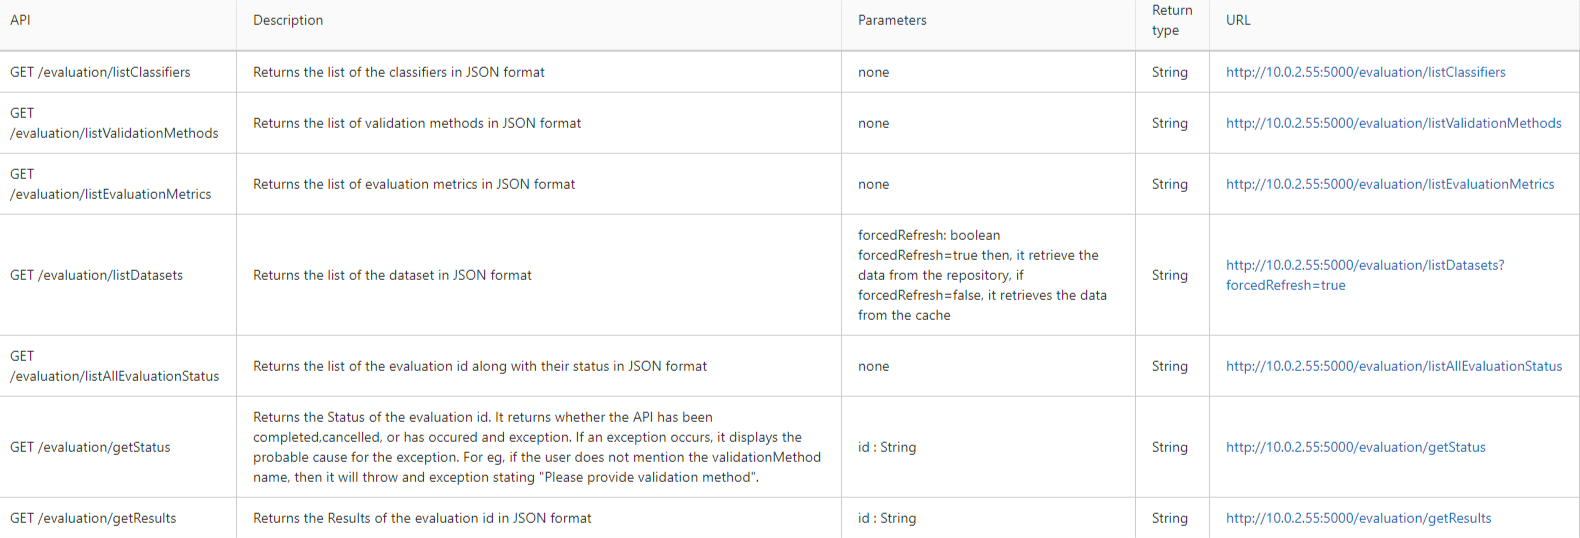
\includegraphics[width=\textwidth]{CodaAPI-GET.png}
	\caption{CODA GET endpoints}
\end{figure}
\begin{figure}
	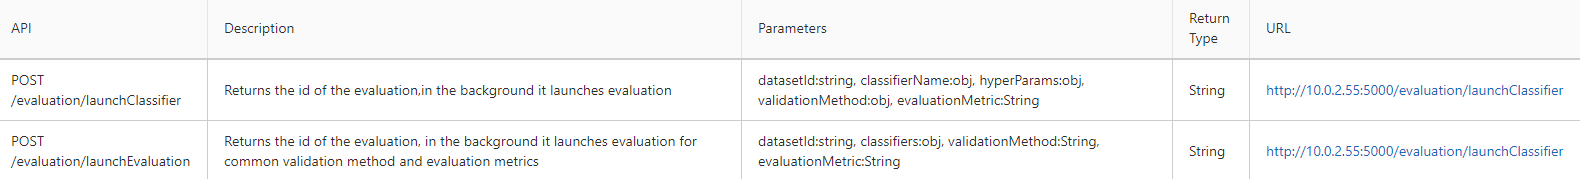
\includegraphics[width=\textwidth]{CodaAPI-POST.png}
	\caption{CODA POST endpoints}
\end{figure}

\section*{Log4j configuration file}
\label{appendix:Log4j}
\begin{lstlisting}[caption={Log4j configuration file.},captionpos=b]
<?xml version="1.0" encoding="UTF-8"?>
<Configuration>
  <Appenders>
    <File name="fileAppender" fileName="logs/log.log">
        <PatternLayout pattern="%d{yyyy-MM-dd HH:mm:ss.SSS} %-5level - %msg%n"/>
    </File>
</Appenders>

  <Loggers>
    <Root level="warn">
    </Root>

    <Logger name="coda.shared" level="debug">
        <AppenderRef ref="fileAppender" />
    </Logger>
  </Loggers>
</Configuration>
\end{lstlisting}
\newpage


